\chapter{Szerver oldali technológiák}\label{ch:szerver}

\begin{osszefoglal}
Az E-migrated alkalmazás szerver oldali komponensének alapja a Java programozási nyelv és a Spring keretrendszer. Ez a fejezet bemutatja a szerver architekturális megoldásait, leírja a különböző rétegeket, a szerver oldalon használt technológiákat,  a komponensek működését és egymással való kommunikációját. 
\end{osszefoglal}

\section{Szerver oldali architekturális megoldások}
\label{sec:szerverArch}

A szerver töbrétegű architekturára épül \cite{MultitierArchitecture}, melynek előnye, hogy a különböző funkciókat megvalósító rétegek egymástól elkülöníthetőek, ezáltal a tőlük függő komponensek módosítása nélkül is lecserélhetőek, illetve a további bővítés és tesztelhetőség is egyszerűen kivitelezhetővé válik. A szerver oldali komponens architekturája \aref{fig:ServerArchitecture}. ábrán látható módon van modularizálva. 
\begin{figure}
  \centering
  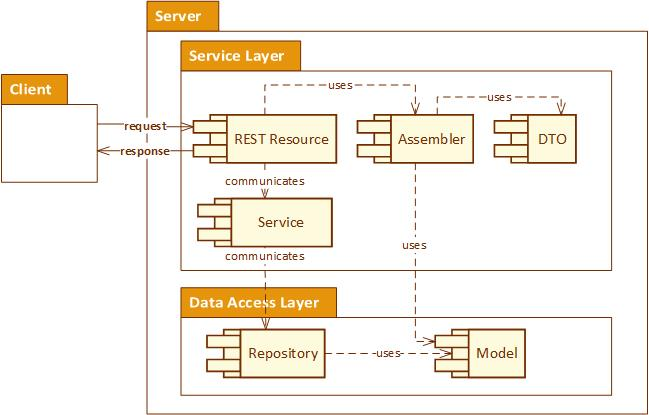
\includegraphics[width=0.9\linewidth]{images/ServerArchitecture}
  \caption{A szerver oldali komponens többrétegű architekturája  az \textit{adathozzáférési rétegből} (Model és Repository) valamint a \textit{szolgáltatási rétegből} (REST Resource, Assembler, DTO és Service) áll.}
  \label{fig:ServerArchitecture}
\end{figure}

Az \textit{adathozzáférési réteg} (data access layer) felelős az adatok perzisztenciájának megvalósításáért, valamint az alacsonyszintű adathozzáférés és az alkalmazás logika elkülönítéséért. Ehhez a réteghez tartoznak a \textit{Model} osztályok, amelyek az alkalmazás fő entitásai, és egyszerű POJO-k (Plain Old Java Object)~\cite{POJO} privát adattagokkal és publikus getter és setter metódusokkal, valamint a \textit{Model} objektumokat használó \textit{Repository} komponens. A \textit{Repository} komponens  által biztosított interfészek segítségével valósul meg a tulajdonképpeni adatkezelés, a DAO (Data Access Object)\cite{DAO} tervezési minta alkalmazásával. Az interfészek használatának előnye, hogy a réteg implementációja bármikor egyszerűen lecserélhető a felsőbb rétegek módosítása nélkül. 

A \textit{szolgáltatási réteg} tartalmazza az alkalmazás logikáját és meghatározza az adatokhoz való hozzáférési lehetőségeket. Az E-migrated projekt esetében ehhez a réteghez tartoznak a \textit{Service}, a \textit{Resource}, az \textit{Assembler}, valamint a \textit{DTO} komponensek. A \textit{Service} komponens használja az adathozzáférési réteg által publikált \textit{Repository} interfészeket és \textit{Model} osztályokat az adatkezeléssel kapcsolatos műveletek megvalósítása érdekében. Köztes szintet képvisel az adathozzáférés és az erőforráspuklikálás között. A szerver által biztosított REST erőforrások közzétételéért és a kliensnek küldött válaszok felépítéséért felelős \textit{Resource} komponens használja a  \textit{Service} és az \textit{Assembler} modulok által közzétett interfészeket, a HTTP protokkolon alapuló kommunikáció megvalósítása érdekében. Az \textit{Assembler} modul végzi az alkalmazás entitásai és a DTO-k közötti átalakítást, így biztosítva, hogy a kliens csak a számára szükséges adatokhoz férhessen hozzá. 




\section{Spring keretrendszer}
\label{subsec:Spring}

A Spring egy összefüggő infrastruktúrát biztosító Java keretrendszer.  Alappillérei az Inversion of Control (IoC) és a Dependency Injection (DI) technikák \cite{IoCDI}, amelyek kezelik és konfigurálják a komponenseket, menedzselik a példányokat és az ezek közötti függőségeket. Ezáltal a Spring leveszi a példányosítás és komplex konstruktormegírás terhét a fejlesztő válláról. Segítségével egy átlátható, moduláris alkalmazás hozható létre, mely klasszikus POJO-kra alapozva biztosítja az enterprise Java szolgáltatásait egy kompakt csomagolásban \cite{Spring}. 

A Spring keretrendszer moduljainak fő csoportja a Core Container~\cite{SpringCore}, amely többek között tartalmazza  a spring-core és spring-beans modulokat, amelyek biztosítják az IoC és DI funkciókat.

Az E-migrated egy Spring-Boot alapú alkalmazás, amely egy egyszerű módszer egy kezdetleges, futtatható Spring alkalmazás felépítésére. Erősségét és népszerűségét annak köszönheti, hogy a "convention over configuration" \cite{Convention} (konvenció konfigurálás fölött) elvet követve, a kezdeti beállításokat, konfigurációkat nem bízza a fejlesztőre, hanem alapértelmezett értéket ad ezeknek, ezáltal elősegítve az alkalmazás egy kezdeti, működő verziójának felépítését. Ez megkönnyíti a külső fejlesztőkkel való kollaborációt is, mert könnyen olvashatóvá teszi a kódot, és a konvenciók számukra is ismerősek lesznek. Természetesen ezek a beállítások a későbbiekben egyszerűen módosíthatóak.\cite{SpringBoot}
\section{Adathozzáférés és adattárolás}
\label{subsec:Adathozzáférés}
Az E-migrated alkalmazás szervere MySQL relációs adatbázist használ az adatok tárolására, amellyel a Spring Data JPA segítségével kommunikál. A Spring keretrendszer az adathozzáférési réteg implementálására egyszerű és kényelmes megoldásokat nyújt. Olyan Data Access Object (DAO) támogatást biztosít, amely által a különböző  perziszenciát biztosító technológiák egységesen és könnyen kezelhetőek (\ref{fig:SpringDataJPA}. ábra). Biztosít egy absztrakciós szintet a  JDBC (Java Database Connectivity) API-hoz, így megkíméli a fejlesztőket a bonyolult, adatbázis specifikus lekérdezések írásától, az alacsonyszíntű részletek implementálásától. Ezen felül biztosít egy egységes hibakezelési módszert, így nem kell külön ismerni a különböző adatbázis specifikus hibákat. 

A \texttt{@Repository} annotáció gondoskodik arról, hogy a komponens szkennelő megtalálja és konfigurálja az adott adathozzáférést biztosító osztályt, így nem szükséges XML állomány a konfigurációk megadására. Az E-migrated alkalmazás esetében is az annotációs megoldás használatos.

A Spring keretrendszer támogatja  a Java Persistence API (JPA) integrációját, amely egy absztrakciós szintet képez a JDBC felett és segítségével szabványosítható az Object Relational Mapping (ORM).  Az ORM célja, hogy megkönnyítse az objektum orientált programozási nyelvek és relációs adatbázisok közötti leképezést \cite{DataAccess}.

Minden Data Access Object-nek vagy adathozzáférést implementáló osztálynak szüksége van egy erőforrás hozzáférést biztosító objektumra, amely a \texttt{@PersistenceContext} annotáció segítségével injektálható be, és amely a META-INF mappában található \textit{persistence.xml} állományban levő konfigurációkkal szabható testre.


 \begin{figure}
  \centering
  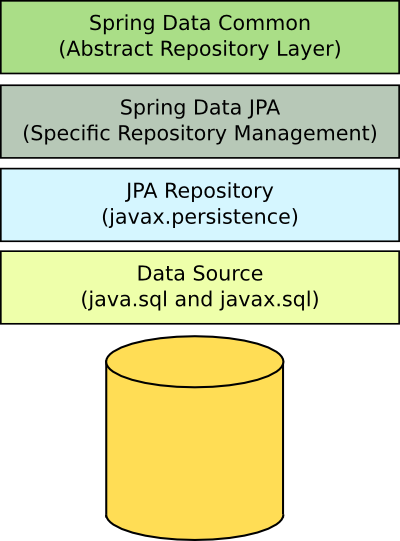
\includegraphics[height=0.5\linewidth]{images/SpringDataJPA}
  \caption{ \protect\footnotemark Spring Data keretrendszer család  lehetővé teszi az adat-hozzáférés egyszerű implementációját, a különböző adattárolási technológiák (pl. SQL és NoSQL adatbázisok) egységes módon való kezelését.}
  \label{fig:SpringDataJPA}
\end{figure}
\footnotetext{Kép forrása: \url{https://visola.github.io/2012/03/26/simple-spring-data-example/index.html}, utolsó megtekintés dátuma: 2018-04-19}

A Spring Data egy keretrendszer család, mely lehetővé teszi az adat-hozzáférés egyszerű implementációját, a különböző adattárolási technológiák (pl. SQL és NoSQL adatbázisok) egységes módon való kezelését. 
A Spring Data repository absztrakció fő interfésze a \texttt{Repository}. A \texttt{CrudRepository} ennek leszármazottja, és lehetővé teszi a CRUD (Create, Read, Update, Delete) műveletek egyszerű megadását. Nem szükséges implementálni a DAO osztályokat, elegendő csupán kiterjeszteni a Spring Data által biztosított interfészeket, és deklarálni a  \texttt{create, read, update, delete} illetve más metódusokat, a keretrendszer a metódus nevéből és a programozó beállításaiból dinamukisan fel tudja építeni a megfelelő adatelérési parancsot \cite{DataJPA}.   Például az  \texttt{InvitationRequestRepository} interfészben a \texttt{findByEmail} metódus, mely visszatéríti a paraméterként megadott e-mail címhez tartozó meghívó kérést, csak ki van jelentve, nincs implementálva, az implementációt a keretrendszer generálja, a betartott konvenciók alapján (\ref{fig:SpringData}. ábra). 
\begin{figure}
  \centering
  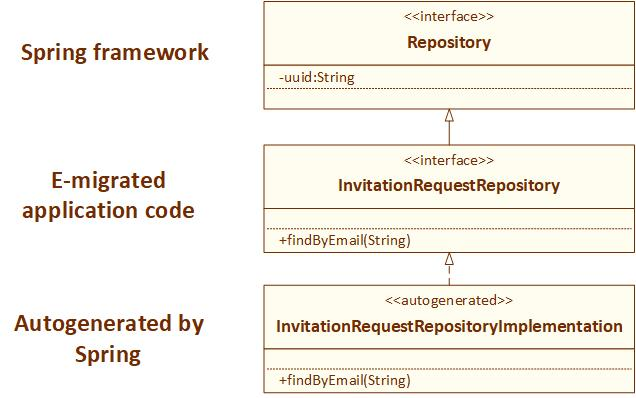
\includegraphics[width=0.7\linewidth]{images/SpringData}
  \caption{A Spring Data keretrendszer leveszi a fejlesztő válláról a DAO osztályok implementációját, elég kiterjeszteni a keretrendszer által biztosított interfészeket és a konvenciókat betartva deklarálni a metódusokat, a Spring a metódus nevéből automatikusan ki tudja generálni az implementációt.}
  \label{fig:SpringData}
\end{figure}

Lehetőség nyílik bonyolultabb lekérdezések egyszerű megadására is \texttt{NamedQuery}-k segítségével. A lekérdezéshez szükséges model osztály definíciója előtt a \texttt{@NamedQuery} annotáció segítségével felépíthető a lekérdezés, akár parametrizálva is. A lekérdezés törzsszövegében használt nyelvezet a  Java Persistence Query Language (JPQL), amelynek segítségével az entity modelre épített adatbázis lekérdezések írhatóak. A JPQL szintaxisa hasonlít az SQL nyelvezetére, de a Java környezetben levő entity osztályneveket használja a lekérdezések felépítésére, nem pedig az adatbázis oldalon levő tábla elnevezéseket.

\begin{listing}
  \inputminted{java}{progfiles/UserRepository.java}
  \caption{Bonyolult lekérdezés megvalósítása a Spring Data keretrendszer és NamedQuery-k segítségével.}
  \label{lst:userRepository}
\end{listing}


Példa erre többek között a \texttt{UserRepository} interfészben, az \ref{lst:userRepository}. kódrészletben található \texttt{findUsersLikeSearch} metódus, amely a \texttt{search} paraméter által megadott szöveg alapján visszatéríti azokat a felhasználókat, akiknek a nevében megtalálható az adott szövegrész. Ez a metódus a többihez hasonlatosan nincsen implementálva, az adatbázis szintű lekérdezést a keretrendszer építi fel, a \texttt{User} model osztálydefiníciója előtt található \texttt{@NamedQuery} annotáció segítségével, amely a \ref{lst:namedQuery}. kódrészletben látható. A \texttt{@Param} annotáció köti össze a \texttt{@NamedQuery}-ben szereplő \texttt{:search} változót a metódus paraméterlistájában szereplő \texttt{search} paraméter értékével. Ennek segítségével bármilyen bonyolult lekérdezés egyszerűen megírható. 

\begin{listing}
  \inputminted[fontsize=\small]{java}{progfiles/UserNamedQuery.java}
  \caption{NamedQuery megadása a User bean osztálydefiníciója előtt, JPQL segítségével.}
  \label{lst:namedQuery}
\end{listing}

A Spring Data \texttt{PagingAndSortingRepository} interfésze olyan esetekben használható amikor nem szükséges, illetve nem kívánatos egyszerre az összes adatbázisban levő objektumot visszatéríteni, csupán azoknak egy részét, például az 10. objektumtól a 15. objektumig. A lapozás megvalósításához elegendő a \texttt{findAll} metódus paraméterének átadni egy \texttt{PageRequest} objektumot, amelynek be van állítva, hogy hányadik oldalt térítse vissza, illetve, hogy egy oldalon hány objektum szerepeljen. Az almalmazáson belül a bejegyzések lapozása van megoldva a \texttt{PagingAndSortingRepository} segítségével.

Az E-migrated adathozzáférési rétegében minden az  \ref{sec:projektrol:adatmodell}. fejezetben említett model osztály  számára létezik egy neki megfelelő \texttt{Repository} interfész. Ezeken kívül még megtalálható a \texttt{UserConnectionRepository}, ami nem leszármazottja a \texttt{Repository} ősinterfésznek, natív implementációt tartalmaz, amire azért volt szükség, hogy a Facebook integráció esetében is biztosítani lehessen a meghíváson alapuló regisztrációt, mivel a Spring Social akkor is létrehoz egy bemenetet a \texttt{UserConnection} táblába, ha valaki illegálisan próbált bejelentkezni. Ezt a rekordot pedig törölni kell, hogy ne kapjon hibát az a személy, aki legálisan, meghívó által próbál regisztrálni az adott Facebook profillal, vagy épp hozzá akarja kötni ezt a Facebook profilt az E-migrated fiókjához.

\section{Üzleti logika réteg}
\label{subsec:szolgaltatas}
Az alkalmazáson belül minden \texttt{Repository} osztályhoz tartozik egy \texttt{@Service} annotációval ellátott Service Spring Bean, amely injektálja a neki megfelelő \texttt{Repository} interfészt, ezáltal hivatkozhat annak metódusaira. Az alkalmazás szolgáltatási rétege a cserélhetőség érdekében egy interfészt publikál az API réteg számára, és ezeket az interfészeket implementálják a \texttt{ServiceImpl} osztályok. Ezáltal az API réteg egyszerűen injektálhatja ezeket az interfészeket, nem kell tudnia a háttérben levő implementációkról. 

A szolgáltatási réteg naplózza, burkolja és továbbítja a kivételeket a felsőbb rétegeknek. Minden szolgáltatási rétegbeli metódus hiba esetén dob egy \texttt{ServiceException}-t amit az API réteg kap el és kezel le.

A \texttt{UserService} osztály kezeli a felhasználókkal kapcsolatos műveleteket, mint például a regisztráció, bejelentkezés, jelszó és felhasználónév módosítás, Facebook által regisztrált felhasználók E-migrated fiókjának létrehozása, valamint visszatéríti a felhasználókat a bejövő paraméterek alapján. 

A \texttt{FacebookConnectionService} osztály hozzájárul a Facebook-kal való regisztráláshoz, illetve egy hagyományosan regisztrált felhasználó E-migrated fiókjának a Facebook profiljával való összekötéséhez (további információ a  \ref{subsec:szocialisHalo}. fejezetben).


\section{API réteg}
\label{subsec:API}

Mivel az API réteg felelős a klienssel való kommunikációért és ezt egy RESTful alkalmazás segítségével teszi meg, kézenfekvő volt használni a Spring által biztosított spring-web csomagot, amely segítségével egyszerűen implementálható egy RESTful alkalmazás. 

\subsection{Spring Web modul}\label{subsubsec:SpringWeb}
A Spring Web modul lehetővé teszi egy Spring keretrendszerre épülő web-alkalmazás létrehozását bonyolult xml állományok nélkül. 

A Spring keretrendszerre épülő RESTful alkalmazások esetében a klienstől érkező kérések kezelését kontrollerek végzik. Egy kontroller a \texttt{@RestController}
annotáció segítségével adható meg. A HTTP kérések kezelőkhöz való rendelését a \texttt{@RequestMapping} annotáció biztosítja, mely meghatározza, hogy egy adott endpoint-ra érkező kérés esetén melyik metódus aktiválódjon.

Az E-migrated alkalmazás esetében a kontrollerek szerepét a \texttt{Resource} osztályok töltik be. Ezek az osztályok injektálják a számukra szükséges szolgáltatás-rétegbeli interfészeket, és ha szükséges továbbítják számukra az adatokat további feldolgozás érdekében.



\subsection{Data Transfer Object}
\label{subsubsec:DTO}
\begin{figure}[!b]
  \centering
  \pgfimage[width=0.9\linewidth]{images/Assembler}
  \caption{Az E-migrated alkalmazás a kliens és a szerver közötti adatmegosztásra DTO-kat használ. A DTO tervezési mintát alkalmazva minden Assembler egy ős Assemblerből származik, és minden Model, illetve DTO rendelkezik egy neki megfelelő Assemblerrel, mely az adott Modelt alakítja át DTO-vá illetve fordítva. A Resource osztályok ezeket az Assemblereket használva dolgozzák fel a beérkező adatatokat. }
  \label{fig:Assembler}
\end{figure}

A kliens és a szerver közötti adatmegosztás Data Transfer Objectek segítségével valósul meg. A DTO-k egyszerű POJO-k, melyek az attribútumaikat beállító és lekérdező getter és setter metódusokat tartalmaznak. A DTO tervezési mintának \cite{DTO} megfelelően minden Transfer Objectnek van egy megfelelő \texttt{Assembler} interfész, amelyek egy közös Assembler interfészből származnak, tehát kötelezően tartalmaznak legalább két metódust (\ref{fig:Assembler}. ábra). A metódusok deklarációjában levő M és D típusnevek egy-egy generikus típust jelölnek, melyet a specifikus \texttt{Assembler} interfészek határoznak meg attól függően, hogy melyik DTO-hoz tartoznak. Az említett metódusok közül az első egy adott \texttt{Model} objektumot alakít át egy neki megfelelő \texttt{DTO}-ra, a második pedig fordítva. 

Azokban az esetekben, ahol szükség volt a klienstől érkező adatok alapján egy \texttt{Model} objektum felépítésére és különböző alapértelmezett értékek beállítására az \texttt{Assembler} osztáyok tartalmaznak egy\texttt{ M create(D dto)} metódust is, amelyek visszatérítenek egy adott \texttt{Model} objektumot. Ilyen például a \texttt{RegistrationUserAssembler} is, ahol egy újonnan regisztrált felhasználónak be kell állítani, hogy kezdetben hány darab meghívóval rendelkezik, valamint az alapértelmezett nyelvet (magyar). Ezeket az alapértelmezett értékeket az \texttt{Assembler} osztály properties állományokból tölti be, hogy egyszerűen, a kód megértése nélkül lehessen változtatni az értéküket. A \texttt{@PropertySource("classpath:application.properties")} annotáció segítségével adható meg, hogy az osztály melyik állományból olvassa az értékeket, illetve az attribútumok deklarálásánál a \texttt{@Value("\${user.defaultNumberOfInvitations}")} annotáció határozza meg, hogy az adott állományból mely mező értékét vegye fel az annotált attribútum.

\section{Biztonsági megoldások}
\label{subsec:biztonsag}
A Spring Security összefogó biztonsági megoldásokat kínál vállalati Java alkalmazások számára. A két fő terület amit a Spring megcéloz a hitelesítés (authentication) és jogosultságellenőrzés (authorization) \cite{SpringSec}. 
A Spring Security testreszabása az alkalmazáson belül a  \texttt{SecurityConfig} osztályban található. Itt történik a felhasználók jelszavainak sózásához és hash-eléséhez szükséges kódolási algoritmus beállítása, amely ebben az esetben a Spring Security által biztosított, napjaink technológiáival visszafejthetetlennek vélt algoritmus, a \texttt{BCryptPasswordEncoder}. A Spring Security megkapja a felhasználó által beírt hitelesítési adatokat, ezeket kódolja, majd összehasonlítja az adatbázisban található hash-elt jelszóval, amennyiben a két jelszó megegyezik a hitelesítés sikeresen megtörtént, különben kivételt dob. 

A rendszeren belül használt \texttt{User} model osztály össze van kötve a Spring Security \texttt{User} osztályával, amely rendelkezik a felhasználónéven és jelszón kívül más attribútumokkal is, melyek további biztonsági ellenőrzéseket tesznek lehetővé, ilyen például az \texttt{accountNonLocked} adattagja. Az E-migrated alkalmazáson belül, ennek segítségével van megoldva, hogy a bejelentkezés sikertelen legyen, amennyiben a felhasználó fiókja fel van függesztve.

\begin{listing}[!b]
  \inputminted[fontsize=\small]{java}{progfiles/security.java}
  \caption{Egy \texttt{HttpSecurity} objektumon keresztül beállítható, hogy mi történjen, ha egy felhasználó nem megfelelő jogosultsággal próbál meg elérni egy erőforrást, illetve testreszabható, hogy mely útvonalak milyen jogosultsággal rendelkező személyek számára legyenek elérhetőek.}
  \label{lst:security}
\end{listing}

A klienstől érkező kérések jogosultságának elbírálását is a \texttt{SecurityConfig} osztályban levő beállítások határozzák meg. Itt van konfigurálva, hogy mi történjen, ha valaki nem megfelelő jogosultsággal próbál elérni egy erőforrást, illetve beállítható, hogy a különböző útvonalak, milyen szerepkörrel rendelkező felhasználók számára legyenek elérhetőek. Ebben a konfigurációs beanben vannak beállítva a sikeres, illetve sikertelen bejelentkezést kezelő útvonalak is (\ref{lst:security}. kódrészlet). 


Az E-migrated esetében az összes \texttt{/guest/**} formájú URL-re érkező kérés mindenkinek elérhető, viszont a \texttt{/user/**} és \texttt{/admin/**} URL-ek alatt levő erőforrásokat csak a megfelelő szerepkörrel rendelkező felhasználók érthetik el. Ugyanez a konvenció vonatkozik az \texttt{/api}-val kezdődő útvonalakra is.

\section{Szociális hálók integrálása}
\label{subsec:szocialisHalo}

Az E-migrated alkalmazásba való regisztráció lehetséges Facebook segítségével, de akár a későbbiekben is hozzákötheti egy felhasználó a Facebook profilját a már meglévő fiókjához. Ennek előnye, hogy nem kell regisztrációs form-ot kitölteni, illetve a bejelentkezés egyszerűbben történik. Az alkalmazás továbbfejlesztésként tervben áll a Google+ és Linkedln integráció is. 


A Spring Social \cite{SpringSocial} célja megkönnyíteni a fejlesztők számára a szociális hálók integrálását a Spring keretrendszerre épülő alkalmazásokba. A Spring Social egy adott felhasználó személyében küld kéréseket a szolgáltató API-jához. A bejelentkezés során a felhasználó a szolgáltató bejelentkezési oldalára lesz átirányítva ahonnan kap egy access tokent. Ez az access token regisztrációkor elmentődik az adatbázisba, tehát az E-migrated szervere ellenőrizni tudja, hogy regisztrált felhasználóról van-e szó. Amennyiben igen, visszatérít neki egy általa generált tokent (az E-migrated szerver esetében a felhasználó nevéből és Facebook ID-jából álló stringet) és ezt követően a felhasználó használhatja az E-migrated szolgáltatásait. 

Azért, hogy az alkalmazásba való regisztráció Facebook-os regisztráció esetében is meghívóhoz legyen kötve, szükséges volt kihasználni a Spring Social rugalmasságát és konfigurálhatóságát. Ennek érdekében a regisztráció során a
 \texttt{/signin/szolgáltató} útvonalra küldött POST kérés különböző rejtett mezőket tartalmaz. Ezekben a rejtett mezőkben kapja meg a szerver többek között a regisztrációs tokent, az email címet amelyre a meghívó volt küldve, illetve annak a személynek az azonosítóját, aki küldte a meghívót. Ezek a rejtett mezők a továbbiakban szesszió hatókörű kérés paraméterekként lesznek továbbítva egészen addig, amíg a szolgáltatótól kapott válasz meg nem érkezik. A válasz érkezése után, a rendszer a kapott válasz és a paraméterek alapján eldönti, hogy sikeres a belépés vagy a regisztráció, vagy nem, illetve ellenőrzi, hogy fel van-e függesztve a felhasználó fiókja. 

A Spring Social konfigurálása a \texttt{SocialConfig} konfigurációs bean-ben történik a csapat által írt adapterek és interceptorok beállításával. 

\section{E-mail küldő mechanizmus}
\label{subsec:e-mail}

Az E-migrated alkalmazás használata során több alkalommal is szükség van e-mail küldésére: meghívó küldése, értesítők kiküldése a profil felfüggesztése illettve újraaktiválása után.

A \texttt{MailSender} a Spring keretrendszer által biztosított fő interfész e-mailek kezelésére. Nagyon sok e-mailküldő rendszer esetében használható egyszerűsége miatt \cite{MailSender}. 

A \texttt{JavaMailSender} interfész a \texttt{MailSender} leszármazottja és ez már lehetőséget nyújt MIME típusú üzenetek küldésére is, általában a \texttt{MimeMessageHelper}-rel együtt használják, amely támogatja különböző csatolmányok (képek, dokumentumok, HTML oldalak) hozzáfűzését a levélhez \cite{JavaMail}. A referencia-implementációja a \texttt{JavaMailSenderImpl} osztály. 

A fejlesztőnek nem kell foglalkozni a Session konfigurálásával sem, a \texttt{JavaMailSender} gondoskodik erről is. Ezen felül biztosít egy kivétel hierarchiát is, melyek mind a \texttt{MailException} leszármozottjai. 

\begin{listing}
  \inputminted[fontsize=\small]{java}{progfiles/SendEmail.java}
  \caption{E-mail küldése a JavaMailSender interfész segítségével.}
  \label{lst:sendEmail}
\end{listing}

Az üzenet felépítése és küldése (\ref{lst:sendEmail}. kódrészlet) során egy \texttt{JavaMailSender} objektum \texttt{createMimeMessage} metódusa által visszatérített \texttt{MimeMessage} megkapja az e-mail elküldéséhez szükséges adatokat, majd a \texttt{send} metódus elküldi az üzenetet. 

Az E-migrated alkalmazás esetében a különböző e-mailek felépítése és elküldése, a \texttt{util} modulon belül levő \texttt{MailSenderBean} osztályban történik. Az e-mail küldéshez szükséges konfigurációs beállítások pedig a \texttt{conf} modulon belül a \texttt{MailSender} konfigurációs osztályban találhatóak meg. Ezeket az értékeket a rendszer egy \texttt{mail.properties} állományból olvassa be a \ref{subsubsec:DTO} fejezetben említett módon. Ebben az állományban található meg többek között az e-mailszerver elérési útvonala és azon belül az alkalmazásnak lefoglalt felhasználónév és jelszó.

A dinamikusan felépített e-mailek renderelése Freemarker templatek alapján történik a Spring Web MVC (Model View Controller) segítségével.



\section{Hibakezelés}
\label{sec:hibakezeles}
A kivételkezelés az alkalmazáson belül rétegenként egységesen va megoldva, mely szerint az alsóbb rétegek naplózzák és burkolják a kivételeket, majd így továbbítják a felsőbb rétegeknek. Az adathozzáférési réteg által dobott kivételeket a szolgáltatási réteg kapja el, és burkolva továbbítja az API rétegnek. Az API réteg kezeli, és HTTP válaszkóddal kiegészítve továbbítja a kliens részére. Ennek előnye, hogy a rétegek egymástól függetlenné válnak, bármikor egyszerűen lecserélhetőek, és a felfele propagáló hibákból a kliens csak annyit lát, amennyire szüksége van, az implementációs részletek rejtve maradnak. 

A Spring Data Access modul segítségével az adathozzáférési réteg által dobott kivételek kezelése általánosan valósítható meg. A keretrendszer naplózza és \texttt{DataAccessException} objektumokba burkolja az ORM illetve a JDBC által dobott specifikus kivételeket. Ezeket  a szolgáltatási réteg elkapja és kezeli, majd \texttt{ServiceException}-ökbe burkolva továbbítja az API rétegnek. A szolgáltatási rétegben fellépő hibák szintén \texttt{ServiceException}-ként lesznek továbbítva a felsőbb komponensnek. 

Az API réteg kommunikál a klienssel, tehát felelős a hibák megfelelő közvetítéséért is. Mivel a szerver a REST princípiumoknak megfelelő JSON formátumú üzenetek segítségével kommunikál a klienssel, hiba fellépése esetén is elvárt, hogy JSON formátumú választ küldjön. Ezért szükséges egy egységes hibakezelési módszer bevezetése, amely elkapja és a kliens számára megfelelő formára térképezi az API rétegben fellépő kivételeket.
\begin{listing}
  \inputminted[fontsize=\small]{java}{progfiles/ApiException.java}
  \caption{A beérkező meghívó igényléseket kezelő metódus \texttt{ApiException}-t dob, ha a csatolt önéletrajz nem PDF formátumban volt feltöltve, illetve abban az esetben is, ha az e-mail küldése során kivétel lép fel. Ezeket a kivételeket az \texttt{ErrorControllerAdvice} kapja el, mappeli és megfelelő formában továbbítja a kliens számára. }
  \label{lst:apiException}
\end{listing}
 \begin{listing}[!b]
  \inputminted[fontsize=\small]{java}{progfiles/ErrorControllerAdvice.java}
  \caption{Az \texttt{ErrorControllerAdvice} figyeli és elkapja a \texttt{@RestController}-ek által dobott kivételeket. Egy figyelni kívánt kivételt a kezelő metódus előtt a  \texttt{@ExceptionHandler} annotáció segítségével vezethetünk be. }
  \label{lst:errorControllerAdvice}
\end{listing}
A REST API kéréseket kezelő \texttt{Resource} osztályok által dobott \texttt{ApiException} példányokat az \texttt{ErrorControllerAdvice} metódusai elkapják, majd a kivétel típusának megfelelő \texttt{ErrorMessageDTO}-t építenek fel, beállítják az odaillő HTTP státuszkódot, végül JSON formátumú választ küldenek a kliensnek. \Aref{lst:apiException}. kódrészletben látható, ahogy a beérkező meghívó igényléseket kezelő metódus \texttt{ApiException}-t dob, ha a csatolt önéletrajz nem PDF formátumban volt feltöltve, illetve abban az esetben is, ha az e-mail küldése során kivétel lép fel. Egy \texttt{ErrorMessageDTO} tartalmazza az üzenet szövegét egy string típusú kulcs formájában, amelyet a kliens oldali fordító értelmez és a megfelelő nyelven jelenít meg.

Az \texttt{ErrorControllerAdvice} egy Java Bean, amely a \texttt{@ControllerAdvice} annotációval van ellátva, ezáltal figyeli és elkapja a \texttt{@RestController}-ek által dobott kivételeket. Egy figyelni kívánt kivételt a kezelő metódus előtt az \texttt{@ExceptionHandler} annotáció segítségével vezethetünk be (\ref{lst:errorControllerAdvice}. kódrészlet). Ez a megoldás lehetővé teszi az összes API rétegben fellépő hiba egyszerű és egységes mappelését. A specifikus hibákon kívül mappelve van az ős \texttt{Exception} osztály is, így biztosítva, hogy bármilyen váratlan hibára megfelelően reagál a szerver. Mivel a kivételeket a kliens \texttt{ErrorMessageDTO}-k formájában kapja meg, az implementációs részletek rejtve maradnak, viszont a számára fontos információ megjelenítésre kerül.  


A Spring Security a jogosultságellenőrzés során fellépő kivételeket statikus hibaoldal visszaküldésével kezeli, amely nem megengedhető egy olyan szerver számára, amely a REST princípiumokat betartva kommunikál a klienssel, így szükségessé válik a keretrendszer által kínált hibakezelési módot testreszabni. Ez többek között a \texttt{SecurityConfig} osztályban valósul meg, ahol egy \texttt{HttpSecurity} objektumon keresztül beállítható, hogy minden hibás jogosultásg esetén a kérés legyen átirányítva az \texttt{/api/accessDenied} endpointra, amelyet az \texttt{AccessDeniedHandler} REST kontroller kezel és megfelelő formában közvetít a kliensnek.
